% Chapter Chapter 8 For Reproducible Research in R and RStudio
% Christopher Gandrud
% Created: 16/07/2012 05:45:03 pm CEST
% Updated: 14 October 2012




\chapter{Statistical Modelling and knitr}\label{StatsModel}

When you have your data cleaned and organized you will begin to examine it with statistical analysis. To make your analysis really reproducible you should dynamically connect the source code of your analysis to your data make file and presentation documents. Connecting to the data make file could involve actually including the code to run your make file in the analysis source code with the \texttt{source} command or if this is computationally intensive you may include this code in the comments so that independent researchers can easily rerun it. Clearly you will directly link to the output of the data gathering make file when you load the data it produced for your statistical analysis. When you dynamically connect your source code file to your markup document you will be able to run your analysis and present the results whenever you compile the presentation documents. Doing this makes it very clear how you found the results that you are advertising. It also automatically keeps the presentation of your results--including tables and figures--up-to-date with any changes you make to your data and analysis.

You can dynamically tie your statistical analyses and presentation documents together with {\emph{knitr}}. In Chapter \ref{GettingStartedRKnitr} you learned basic {\emph{knitr}} syntax. In this chapter you will begin to learn {\emph{knitr}} syntax in much more detail, particularly code chunk options for including dynamic code in your presentation documents. This includes code that is run in the background, i.e. not shown in the presentation document as well as displaying the code and output in your presentation document both as separate blocks and inline with the text. You will also learn how to dynamically include code from languages other than R. We will finally examine how to use {\emph{knitr}} when you segment your analysis into a number of modular source code files. 

The goal of this and the next two chapters--which cover dynamically presenting results in tables and figures--is to show you how to tie your analyses into your presentation documents so closely that every time the documents are compiled they actually reproduce your analysis and present the results.

Please see the next part of this book, Part IV, for details on how to create the LaTeX and Markdown documents that can include {\emph{knitr}} code chunks.

\section{Incorporating analyses into the markup}

For a relatively short piece of code that you don't need to run in multiple presentation documents it may be simplest to type the code directly into chunks written in your markup document. In this section you will learn how set {\emph{knitr}} options to handle these code chunks.

\subsection{Full code chunks}

By default {\emph{knitr}} code chunks are run by R, the code and any text output (including warnings and error messages) are inserted into the text of your presentation documents in blocks. The blocks are positioned in the final presentation document text exactly where they are written in the markup version. Figures are inserted as well. Let's look at the main options for determining how R code is handled by {\emph{knitr}}.

\paragraph{{\tt{eval}}}\index{eval}

Set the \texttt{eval} option to \texttt{FALSE} if you would like to include code chunks without actually running them.

\paragraph{{\tt{echo}}}\index{echo}

The opposite of \texttt{eval=FALSE} is to have the code chunk evaluated but have the code not included in the presentation document. You can do this by setting \texttt{echo=TRUE}. You will use this option extensively in chapters \ref{TablesChapter} and \ref{FiguresChapter} when you learn how to run R source code to produce tables and figures that are included presentation documents' text.

\paragraph{{\tt{warning}}, {\tt{message}}, {\tt{error}}}\index{warning}\index{error}\index{message}

If you don't want to include in the text of your presentation documents the warnings, messages, and error messages that R outputs when it runs a code chunk just set the \texttt{warning}, \texttt{message}, and \texttt{error} options to \texttt{FALSE}.

\paragraph{{\tt{cache}}}\index{cache}

If you want to store a code chunk's output for use later, rather than running the code chunk every time you compile your presentation document, set the option \texttt{cache=TRUE}. When you do this the code chunk is run only if the code changes. It is very handy if you have a code chunk that is computationally intensive to run. 

Unfortunately, the \texttt{cache} option has some limitations. For example, other code chunks can't access objects that have been cached.

\subsection{Showing code \& results inline}

Sometimes you may want to have some R code or text output show up inline with the rest of your presentation document's text. For example, you may want to include a small chunk of stylized code in your text when you discuss how you did an analysis. Or you may want to dynamically report the mean of some variable in your text so that the text will change if you change the data. The {\emph{knitr}} syntax for including inline code is different for the LaTeX and Markdown languages. We'll cover both in turn.

\subsubsection{LaTeX}

\paragraph{Inline static code}

If you want to include a code snippet inline with your text you can simply use the LaTeX command  \texttt{\textbackslash{}texttt}\index{tt}. This sets your text to `typewriter' font, the standard font for inline code in LaTeX (I use it in this book, as you have probably noticed). It is equivalent to the \texttt{eval=FALSE} option for full code chunks. 

\paragraph{Inline dynamic code}

If you want to dynamically show the results of some R code in your LaTeX produced text you can use the  \texttt{\textbackslash Sexpr} command\index{Sexpr}. This is a pseudo LaTeX command; it looks like LaTeX, but is actually {\emph{knitr}}.\footnote{The command directly descends from Sweave.} Its structure is more like a LaTeX command's structure than \texttt{knitr}'s in that you enclose your R code in curly brackets (\texttt{\{\}}) rather than the usual \texttt{\textless\textless\textgreater\textgreater= . . . @} syntax for block code chunks.

For example, imagine that you wanted to include the mean of a vector of river lengths--591--in the text of your document. The {\emph{rivers}} numeric vector, loaded by default in R, has the length of 141 major rivers recorded in miles. You can simply use the {\tt{mean}} command to find the mean and the {\tt{round}} command to round it to the nearest whole number:

\begin{knitrout}
\definecolor{shadecolor}{rgb}{0.969, 0.969, 0.969}\color{fgcolor}\begin{kframe}
\begin{alltt}
\hlfunctioncall{round}(\hlfunctioncall{mean}(rivers), digits = 0)
\end{alltt}
\begin{verbatim}
## [1] 591
\end{verbatim}
\end{kframe}
\end{knitrout}


\noindent To have just the output show up inline with the text of your document you would type something like:

\begin{knitrout}
\definecolor{shadecolor}{rgb}{0.969, 0.969, 0.969}\color{fgcolor}\begin{kframe}
\begin{alltt}
The mean length of 141 major rivers in North America
is \textbackslash{}Sexpr\{\hlfunctioncall{round}(\hlfunctioncall{mean}(rivers), digits = 0)\} miles. 
\end{alltt}
\end{kframe}
\end{knitrout}


\noindent This produces the sentence:

\begin{quote}
    The mean length of 141 major rivers in North America is 591 miles. 
\end{quote}

\subsubsection{Markdown}

\paragraph{Inline static code}

To include static code inline in an R Markdown (and regular Markdown) document, enclose the code in single backticks (\` \`). For example:

\begin{knitrout}
\definecolor{shadecolor}{rgb}{0.969, 0.969, 0.969}\color{fgcolor}\begin{kframe}
\begin{alltt}
This is example R code: `MeanRiver <- \hlfunctioncall{mean}(rivers)`.
\end{alltt}
\end{kframe}
\end{knitrout}


\noindent produces:\footnote{The exact look of the text depends on the CSS\index{CSS} style file you are using.}


\includegraphics[scale = 0.6]{/git_repositories/Rep-Res-Book/Source/Children/Chapter8/images8/MeanRiverMarkdown.png}

\paragraph{Inline dynamic code}

Including dynamic code in the body of your R Markdown text is similar to including static code. The only difference is that you put the letter \texttt{r} after the first single backtick. For example:

\begin{knitrout}
\definecolor{shadecolor}{rgb}{0.969, 0.969, 0.969}\color{fgcolor}\begin{kframe}
\begin{alltt}
`r \hlfunctioncall{mean}(rivers)`
\end{alltt}
\end{kframe}
\end{knitrout}


\noindent will include the mean value of the {\emph{rivers}} vector in the text of your Markdown document.

\subsection{Dynamically including non-R code}

You are not limited to dynamically including just R code in your presentation documents. {\emph{knitr}} can run code from a variety of other languages including: Python\index{Python}, Ruby, Bash, Haskell, and Awk. All you have to do to dynamically include code from one of these languages is set the \texttt{engine}\index{engine} code chunk option. For example, to dynamically include a simple line of Ruby code in an R Markdown document simply type:

\begin{knitrout}
\definecolor{shadecolor}{rgb}{0.969, 0.969, 0.969}\color{fgcolor}\begin{kframe}
\begin{verbatim}
```{r engine='ruby'}
print "Reproducible Research"
 

Reproducible Research
```
\end{verbatim}
\end{kframe}
\end{knitrout}

The programming language values \texttt{engine} can take are listed in Table \ref{EngineOptions}. Please note that currently the range of functions {\emph{knitr}} supports for these languages is less extensive than what it supports for R. For example, there is no colored syntax highlighting.

\section{Dynamically including modular analysis files}

There are a number of reasons that you might want to have your R source code located in separate files from your markup documents even if you compile them together with {\emph{knitr}}.

\begin{wraptable}{rt}{0.4\textwidth}
    \caption{Knitr \texttt{engine} Values}
    \label{EngineOptions}
    \begin{tabular}{l p{2.25cm}}
    \hline\vspace{0.15cm}
    Value & Programming Language \\
    \hline\hline
    \texttt{awk} & Awk\index{Awk} \\
    \texttt{bash} & Bash\index{Bash} \\
    \texttt{gawk} & Gawk\index{Gawk} \\
    \texttt{haskell} & Haskell\index{Haskell} \\
    \texttt{highlight} & Highlight\index{Highlight, knitr engine option} \\ 
    \texttt{python} & Python\index{Python} \\
    \texttt{R} & R (default) \\[0.25cm]
    \texttt{ruby} & Ruby\index{Ruby} \\
    \texttt{sh} & Bash \\
    \hline
    \end{tabular}
\end{wraptable}

First, it can be unwieldy to edit both your markup and long R source code chunks in the same document, even with RStudio's handy {\emph{knitr}} code folding and chunk management options. There are just too many things going on in one document. 

Second, you may want to use the same code in multiple documents--an article and presentation for example. It is nice to not have to copy and paste the same code into multiple places. Instead it is easier to have multiple documents link to the same source code. When you make changes to this source code files, the changes will automatically be made across all of your presentation documents. You don't need to make the same changes multiple times.

Third, other researchers trying to replicate your work might only be interested in specific parts of your analysis. If you have the analysis broken into separate and clearly labeled modular files that are explicitly tied together in the markup file with {\emph{knitr}} it is easy for them to find the specific bits of code that they are interested in.

\subsection{Source from a local file}

Usually in the early stages of research you may want to run code stored in analysis files located on your computer. Doing this is simple. The {\emph{knitr}} syntax is the same as for block code chunks. The only change is that instead of writing all of your code in the chunk you save it to its own file and use the \texttt{source} command to access it. For example, in an R Markdown file we could run the R code in a file called {\emph{MainAnalysis.R}} from our {\exmph{ExampleProject}} like this:

\begin{knitrout}
\definecolor{shadecolor}{rgb}{0.969, 0.969, 0.969}\color{fgcolor}\begin{kframe}
\begin{alltt}
```\{r, echo=FALSE\}
\hlcomment{# Run main analysis}
\hlfunctioncall{source}(\hlstring{"/ExampleProject/Analysis/MainAnalysis.R"}\}
```
\end{alltt}
\end{kframe}
\end{knitrout}


Notice that we set the \texttt{echo=FALSE} option. This will run the analysis and produce objects created by the analysis code that can be used by other code chunks, but the results are not show in the presentation document's text. Errors, messages, and warnings will be shown, if we do not tell {\emph{knitr}} to hide them.

\subsection{Source from a non-secure URL (\texttt{http})}

Sourcing from your computer is fine if you are working alone and do not want others to access your code. Once you start collaborating and generally wanting people to be able to reproduce your analyses, you need to
use another storage method.%\footnote{You can make the replication code accessible for download and either instruct others to change the working directory to the replication file or have them change the directory information as necessary. However, this usually just adds an extra complicating step that makes replication harder. It is also a pain if you are collaborating and each author has to constantly change the directories.}

The simplest solution to these issues is to host the replication code in your Dropbox public folder. You can find the file's public URL the same that you did in Chapter \ref{Storing}. Now use the \texttt{source} command the same way as before with the URL as the argument.

\subsection{Source from a secure URL (\texttt{https})}

If you are using GitHub\index{GitHub} or another service that uses secure URLs to host your analysis source code files you need to use the \texttt{source\_url} command in the {\emph{devtools}} package \cite[]{R-devtools}. For GitHub based source code we find the file's URL the same way we did in Chapter \ref{Storing}. Remember to use the URL for the {\emph{raw}} version of the file. I have a short script hosted on GitHub for creating a scatterplot from data in R's {\emph{cars}} data set. The script's shortened URL is \url{http://bit.ly/Ny1n6b}.\footnote{The original URL is at \url{https://raw.github.com/christophergandrud/christophergandrud.github.com/master/SourceCode/CarsScatterExample.R}. This is very long, so I shortened it using bitly (see \url{http://bitly.com}). You may notice that the shortened URL is not secure. However, it does link to original secure {\tt{https}} URL.} To run this code and create the scatterplot using {\tt{source\_url}} you simply type:

\begin{knitrout}
\definecolor{shadecolor}{rgb}{0.969, 0.969, 0.969}\color{fgcolor}\begin{kframe}
\begin{alltt}
\hlcomment{# Load library}
\hlfunctioncall{library}(devtools)

\hlcomment{# Run the source code to create the scatter plot}
\hlfunctioncall{source_url}(\hlstring{"http://bit.ly/Ny1n6b"})
\end{alltt}
\end{kframe}

{\centering 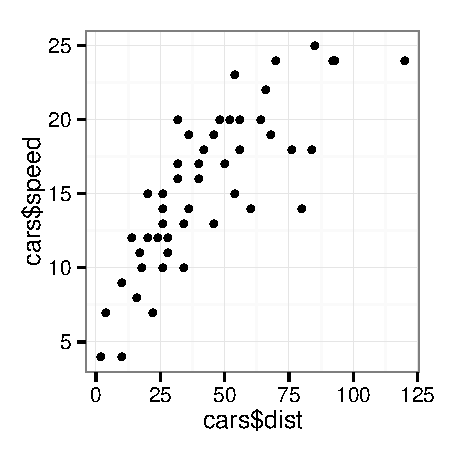
\includegraphics[width=\maxwidth]{figure/Ch8SourceURLExample} 

}


\end{knitrout}


You can also use the {\emph{devtools}} command \texttt{source\_gitst}\index{source\_gist} in a similar way to source GitHub Gists\index{Gist, GitHub}. Gists are a handy way to share code over the internet. For mor details see: \url{https://gist.github.com/}.

